%% March 2018
%%%%%%%%%%%%%%%%%%%%%%%%%%%%%%%%%%%%%%%%%%%%%%%%%%%%%%%%%%%%%%%%%%%%%%%%%%%%
% AGUJournalTemplate.tex: this template file is for articles formatted with LaTeX
%
% This file includes commands and instructions
% given in the order necessary to produce a final output that will
% satisfy AGU requirements, including customized APA reference formatting.
%
% You may copy this file and give it your
% article name, and enter your text.
%
%
% Step 1: Set the \documentclass
%
% There are two options for article format:
%
% PLEASE USE THE DRAFT OPTION TO SUBMIT YOUR PAPERS.
% The draft option produces double spaced output.
%

%% To submit your paper:
\documentclass[draft,linenumbers]{agujournal2018}
\usepackage{apacite}
\usepackage{url} %this package should fix any errors with URLs in refs.
%%%%%%%
% As of 2018 we recommend use of the TrackChanges package to mark revisions.
% The trackchanges package adds five new LaTeX commands:
%
%  \note[editor]{The note}
%  \annote[editor]{Text to annotate}{The note}
%  \add[editor]{Text to add}
%  \remove[editor]{Text to remove}
%  \change[editor]{Text to remove}{Text to add}
%
% complete documentation is here: http://trackchanges.sourceforge.net/
%%%%%%%


%% Enter journal name below.
%% Choose from this list of Journals:
%
% JGR: Atmospheres
% JGR: Biogeosciences
% JGR: Earth Surface
% JGR: Oceans
% JGR: Planets
% JGR: Solid Earth
% JGR: Space Physics
% Global Biogeochemical Cycles
% Geophysical Research Letters
% Paleoceanography and Paleoclimatology
% Radio Science
% Reviews of Geophysics
% Tectonics
% Space Weather
% Water Resources Research
% Geochemistry, Geophysics, Geosystems
% Journal of Advances in Modeling Earth Systems (JAMES)
% Earth's Future
% Earth and Space Science
% Geohealth
%
% ie, \journalname{Water Resources Research}

\journalname{JGR: Atmospheres}

\usepackage{gensymb}
\usepackage{trackchanges}

\begin{document}

%% ------------------------------------------------------------------------ %%
%  Title
%
% (A title should be specific, informative, and brief. Use
% abbreviations only if they are defined in the abstract. Titles that
% start with general keywords then specific terms are optimized in
% searches)
%
%% ------------------------------------------------------------------------ %%

% Example: \title{This is a test title}

\title{Are quasi-stationary waves and planetary waves the same?}

%% ------------------------------------------------------------------------ %%
%
%  AUTHORS AND AFFILIATIONS
%
%% ------------------------------------------------------------------------ %%

% Authors are individuals who have significantly contributed to the
% research and preparation of the article. Group authors are allowed, if
% each author in the group is separately identified in an appendix.)

% List authors by first name or initial followed by last name and
% separated by commas. Use \affil{} to number affiliations, and
% \thanks{} for author notes.
% Additional author notes should be indicated with \thanks{} (for
% example, for current addresses).

% Example: \authors{A. B. Author\affil{1}\thanks{Current address, Antartica}, B. C. Author\affil{2,3}, and D. E.
% Author\affil{3,4}\thanks{Also funded by Monsanto.}}

\authors{
Elio Campitelli
\affil{1}
Carolina Vera
\affil{1, 2}
Leandro Díaz
\affil{1, 2}
}


% \affiliation{1}{First Affiliation}
% \affiliation{2}{Second Affiliation}
% \affiliation{3}{Third Affiliation}
% \affiliation{4}{Fourth Affiliation}

\affiliation{1}{Centro de Investigaciones del Mar y la Atmosfera, UMI-IFAECI
(CONICET-UBA-CNRS)}
\affiliation{2}{Departamento de Ciencias de la Atmósfera y los Océanos (FCEyN, UBA)}
%(repeat as many times as is necessary)

%% Corresponding Author:
% Corresponding author mailing address and e-mail address:

% (include name and email addresses of the corresponding author.  More
% than one corresponding author is allowed in this LaTeX file and for
% publication; but only one corresponding author is allowed in our
% editorial system.)

% Example: \correspondingauthor{First and Last Name}{email@address.edu}
\correspondingauthor{Elio Campitelli}{elio.campitelli@cima.fcen.uba.ar}

%% Keypoints, final entry on title page.

%  List up to three key points (at least one is required)
%  Key Points summarize the main points and conclusions of the article
%  Each must be 100 characters or less with no special characters or punctuation

% Example:
% \begin{keypoints}
% \item	List up to three key points (at least one is required)
% \item	Key Points summarize the main points and conclusions of the article
% \item	Each must be 100 characters or less with no special characters or punctuation
% \end{keypoints}

\begin{keypoints}
\item List up to three key points (at least one is required)
\item Key Points summarize the main points and conclusions of the article
\item Each must be 100 characters or less with no special characters or
punctuation
\end{keypoints}

%% ------------------------------------------------------------------------ %%
%
%  ABSTRACT
%
% A good abstract will begin with a short description of the problem
% being addressed, briefly describe the new data or analyses, then
% briefly states the main conclusion(s) and how they are supported and
% uncertainties.
%% ------------------------------------------------------------------------ %%

%% \begin{abstract} starts the second page

\begin{abstract}
A good abstract will begin with a short description of the problem being
addressed, briefly describe the new data or analyses, then briefly
states the main conclusion(s) and how they are supported and
uncertainties.
\end{abstract}

\section{Introduction}

Atmospheric planetary waves are blabalbaal\ldots{} In some latitudes and
tiems of the year they exhibit some degree of stationatiry\ldots{}

\section{Story}

\ldots{}

Zonal waves (ZW; sometimes also called planetary waves) are waves
observed in each individual ``instantaneous'' field. Quasi-stationary
waves (QS), on the other hand, are the resulting waves in the mean
field. Of course, these definitions depend on which are the
``instantaneous field'' in question and the averaging timescales used.
However, they illustrate that, given a set of fields, ZWs are properties
of the \emph{elements} of the set, while the QS is a property of the set
as a whole. This is an important distinction with theorical and
methodological implications but is not always appreciated in the
literature.

\begin{figure}[h]
\includegraphics{fig/QS-ZW/rao-1} \caption{Seasonal cycle of amplitude of the geopotential planetary waves 1 to 3 at 60\degree S computed as the mean amplitude of the monthly waves ($\overline{ZW}$) and as the amplitude of the mean wave (QS). The period of analysis is 1950 to 1998. The left column reproduces Figure 3 from \citet{Rao2004}.}\label{fig:rao}
\end{figure}

As an example, Figure \ref{fig:rao} shows the monthly seasonal cycle of
amplitude of planetary waves at 60\degree S using monthly fields from
the NCEP/NCAR reanalysis \citep{Kalnay1996} between 1950 and 1998. The
left column (\(\overline{ZW}\)) reproduces Figure 3 from \citet{Rao2004}
and is computed by taking --for each month and level-- the average
amplitude of the 49 individual amplitudes. The right column (QS), on the
other hand, is computed by taking the amplitude of the average
geopotential field for each month and level.

The resulting fields convey different information. First, the amplitude
of \(\overline{ZW}\) fields is always greater than the one for QS
fields. This is a
\annote[elio]{mathematical necessity}{Deberia demostrar eso? Vale la pena una demostracion en un material suplementario?}
that explains \citet{Rao2004}'s observation that their Wave 1 amplitude
was greater than that reported by \citet{Hurrell1998}. Secondly, they
have different annual cycles and vertical structures. QS2, for example,
has a strong minimum in the low stratosphere during the austral autumn
that is not aparent in \(\overline{ZW2}\). Similarly, the austral winter
mid-troposferic maxmium is very well defined in \(\overline{ZW3}\) but
not so in QS3. Thirdly, the relative importance between each wavenumber
vary. \(\overline{ZW}\) fields show, for example, a preponderance of
wave 2 over 3 in almost every level and month. However, the QS3 has
greater amplitude than QS2 in the first half of the year. In contrast
with wave-numbers 2 and 3, \(\overline{ZW1}\) and QS1 fields are very
similar.

\begin{figure}[h]
\includegraphics{fig/QS-ZW/hurrell-1} \caption{Seasonal cycle of amplitude of the geopotential planetary waves 2 at 300hPa computed as the mean amplitude of the monthly waves ($\overline{ZW}$) and as the amplitude of the mean wave (QS). The period of analysis is 1979 to 2017.}\label{fig:hurrell}
\end{figure}

These differences are related to the degree of stationatiry of zonal
waves and are location-dependent. Figure \ref{fig:hurrell} show the same
variable that Figure \ref{fig:rao} but for 300hPa. The contrast between
the northern and shouthern hemisphere is not only evident in the
amplitud of the planetary waves, but also in the comparison between
\(\overline{ZW}\) and QS. Specially for wave-numbers 2 and 3,
\(\overline{ZW}\) and QS fields are very similar in the north but they
have significant diferences in the south. The theorical implication is
that planetary waves are more stationary in the northern hemispher while
the practical implication is that researchers of the southern hemisphere
planetary waves should be specially atentive to the choice of
metodology.

Another important consequence of the distinction between
\(\overline{ZW}\) and QS is that the quotient between the two can be
used as a measure of stationarity. As an analogy with the steadiness of
the wind \citep{Singer1967}, planetary wave stationarity can be
calculated as

\begin{linenomath*}
\begin{equation}
S = \frac{2}{\pi}\arcsin{\left ( \frac{QS}{\overline{ZW}} \right )}
\end{equation}
\end{linenomath*}

It can be shown that \(S = 1\) for completely stationary waves and that
\(\lim_{n \rightarrow \inf} S = 0\) for completely non-stationary waves
with convergence of \(O\left (n^{1/2}\right)\) (where \(n\) is the
sample size).

\begin{figure}[h]
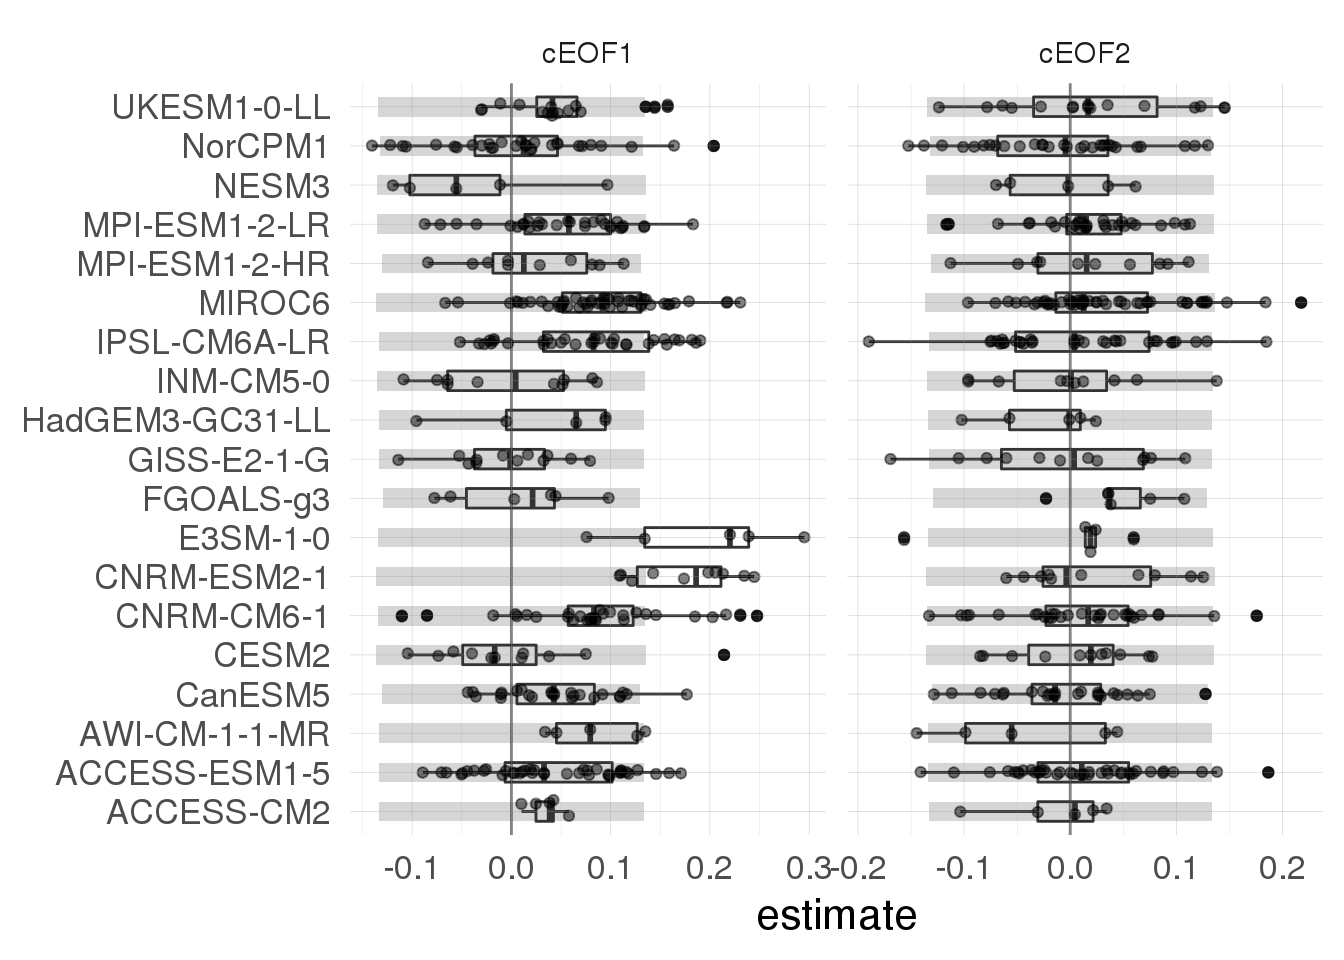
\includegraphics{fig/QS-ZW/unnamed-chunk-1-1} \caption{Please caption every figure}\label{fig:unnamed-chunk-1}
\end{figure}

\subsection{Mathematical considerations}

Let \(w_1\), \(w_2\) be two waves of wavenumber \(k\) defined by

\begin{linenomath*}
\begin{equation}
w_1 = A_1\cos(k(\phi - \alpha_1)) \quad
w_2 = A_2\cos(k(\phi - \alpha_2)) 
\end{equation}
\end{linenomath*}

where \(A_i\), \(alpha_i\) are their amplitudes and phases and \(\phi\)
is longitude. The amplitude of the sum of both waves is

\begin{linenomath*}
\begin{equation}
A(w_1 + w_2) = A_3 = \sqrt{A_1^2 + A_2^2 + 2A_1A_2\cos(\alpha_1 - \alpha_2)}
\end{equation}
\end{linenomath*}

\bibliography{qszw.bib}


\end{document}
